\documentclass[../diploma.tex]{subfiles}
 
\begin{document}

	\label{sec:methods_and_implementation}

	\subsection{Извлечение признаков}

	Напомним, что после предобработки датасета мы получили данные, 
	в которых присутсвуют тексты ответа и вопроса, к которому относится текущий ответ, а также некоторая метаинформация.

	Нейронные сети работают с числовыми признаками, 
	поэтому в следующих подразделах будет, во-первых, описан использованный подход к векторизации слов, 
	а во-вторых, перечислены дополнительные признаки, которые могут помочь в поставленной перед нами задаче классификации.

	\subsubsection{Векторное представление вопроса и ответа}

   	Как уже говорилось в подразделе \ref{subsec:word_embedding}, существует несколько способов векторизации слов,
   	но нас будут интересовать Word2Vec и Fasttext, которые помимо прочего хорошо описывают семантику слов.

   	Для обучения этих алгоритмов требуется большой корпус неразмеченных данных, 
   	в нашей работе использовалось обучение на базе данных \cite{online:wiki_dump}, состоящей из статей Wikipedia до октября $2017$ года.
   	В этом корпусе присутствует $\approx 4.9$ миллиона статей, в которых содержатся $\approx 132$ миллиона предложений и $\approx 2.5$ миллиарда слов.
   	При обучении игнорировались слишком короткие предложения (длиной менее $5$), а также использовалась модель CBOW.

   	В связи со спецификой Server Fault в текстах вопросов и ответов встречается множество технических слов и терминов, 
   	кроме того, как и на любом форуме, часто пользователи пишут слова с ошибками или опечатками.
   	Это приводит к тому, что модель Word2Vec, обученная по корпусу Wikipedia, не содержит множества слов, присутствующих в текстах вопросов и ответов, 
   	в том числе терминов, которые являются важной информацией. В среднем, модель не содержала векторных представлений $\approx 10$ слов на каждую пару вопроса и ответа.

   	Чтобы это исправить, было предпринято два шага: 
   	
   	\begin{itemize}
   		\item
   		Так как часто новые слова являются конкатенацией слов из словаря, например, \textit{texthtml} или \textit{powercenter}, 
   		а слова с опечатками отличаются от слов из словаря всего одним символом, 
   		то есть множество $n$-грамм у них сильно пересекается с множеством $n$-грамм слов из словаря,
       	то вместо использования Word2Vec мы решили использовать модификацию, которая работает с $n$-граммами~--- Fasttext.

   		\item
   		Также у нас есть специализированные тексты, которые можно использовать для обучения нашей модели, поэтому 
   		модель была дотренирована на текстах вопросов и ответов из обучающей подвыборки.

   	\end{itemize}

   	Английский~--- аналитический язык, что значит, что в нем грамматические отношения передаются через синтаксис, то есть через отдельные служебные слова.
   	Например, в отличие от синтетического русского языка в нем нет склонений.

   	А исходя из того, что корпус текстов Wikipedia большой, то отпадает потребность производить стемминг, который наоборот может лишь ухудшить качество векторизации, 
   	склеивая несколько различных слов в одно.

	\subsubsection{Лингвистические признаки}

   	Кроме содержания, часто важно и грамотное оформление ответа: логичное разбиение на предложения и параграфы, проставленные ссылки на источники и удобочитаемость.
   	Поэтому в качестве дополнительных лингвистических были извлечены следующие признаки, описывающие либо структуру \texttt{HTML}-кода, либо текста ответа:

   	\begin{itemize}
   		\item
   		Количество ссылок в тексте, то есть количество тегов \texttt{<a>}.

   		\item
   		Количество фрагментов кода в тексте, то есть количество тегов \texttt{<code>}.

   		\item
   		Количество параграфов в тексте, то есть количество тегов \texttt{<p>}.

   		\item
   		Доля заглавных букв в тексте, то есть отношение количества заглавных букв к длине текста.

   		\item
   		Доля строчных букв в тексте, то есть отношение количества строчных букв к длине текста.

   		\item
   		Доля пробелов в тексте, то есть отношение количества пробельных символов к длине текста.

   		\item
   		Длина текста.

   		\item
   		Длина самого длинного предложения.

   		\item
   		Количество слов в самом длинном предложении.

   		\item
   		Среднее количество слов в предложении.

   		\item
   		Средняя длина слова в тексте.

   		\item
   		Количество предложений.

   		\item
   		Автоматический индекс удобочитаемости \cite{article:ari}: 
   		\begin{equation} 
   			ARI = 4.71 \cdot \frac{characters}{words} + 0.5 \cdot \frac{words}{sentences} - 21.43
   		\end{equation}

   		\item
   		Индекс удобочитаемости Флеша \cite{article:fre}: 
   		\begin{equation} 
   			FRE = 206.835 - 1.015 \cdot \frac{words}{sentences} - 84.6 \cdot \frac{syllables}{words}
   		\end{equation}

   		\item
   		Индекс \texttt{SMOG} \cite{article:smog}: 
   		\begin{equation}
   			SMOG = 1.043 \cdot \sqrt{\frac{30 \cdot polysyllables}{sentences}} + 3.1291
   		\end{equation}

   		\item
   		Индекс Флеша-Кинкейда \cite{article:fk}: 
   		\begin{equation}
   			FK = 0.39 \cdot \frac{words}{sentences} + 11.8 \cdot \frac{syllables}{words} - 15.59
   		\end{equation}
   	
   		\item
   		Индекс Колман-Лиау \cite{article:cli}: 
   		\begin{equation}
   			CLI = 5.88 \cdot \frac{characters}{words} - 29.6 \cdot \frac{sentences}{words} - 15.8
   		\end{equation}
   		
   		\item
   		Фог-индекс \cite{book:fog}: 
   		\begin{equation}
   			FOG = 0.4 \cdot \left( \frac{words}{sentences} + 100 \cdot \frac{polysyllables}{words} \right)
   		\end{equation}

   		\item
   		Индекс \texttt{LIX} \cite{book:lix}: 
   		\begin{equation}
   			LIX = \frac{words}{sentences} + 100 \cdot \frac{longwords}{words}
   		\end{equation}
   	
   	\end{itemize}
    
    В упомянутых выше формулах использованы следующие обозначения:
    
    \begin{itemize}
    	\item
    	$characters$~--- количество символов в тексте,

	    \item
	   	$words$~--- количество слов в тексте,

	    \item
	   	$sentences$~--- количество предложений в тексте,

	    \item
	   	$syllables$~--- количество слогов в тексте,

	    \item
	   	$polysyllables$~--- количество слов с хотя бы тремя слогами,

	    \item
	   	$longwords$~--- количество слов длины хотя бы $7$.
	\end{itemize}

   	На рисунке \ref{fig:lix_index} можно увидеть распределение значений индекса удобочитаемости \texttt{LIX} правильных и неправильных ответов, 
   	из которого видно, что подобные индексы действительно влияют на решение пользователя о выборе правильного ответа.

   	\vskip 1em
    \begin{figure}[ht]
   	    \centering
		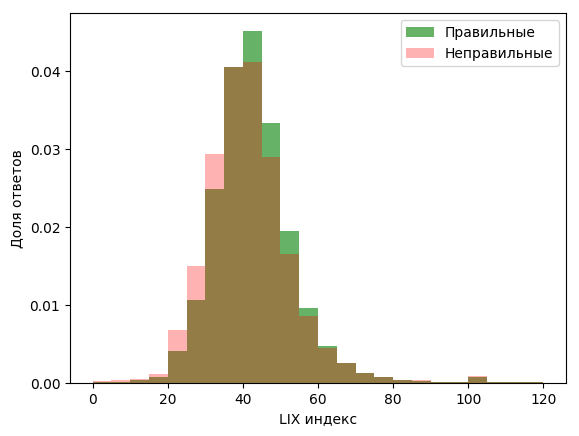
\includegraphics[width=0.9\linewidth]{images/lix.png}
   		\captionof{figure}{Распределение значений индекса \texttt{LIX}}
		\label{fig:lix_index}
   	\end{figure}

	\subsubsection{Словарные признаки}

   	Как было замечено ранее, в текстах встречается множество терминов, 
   	поэтому для оценки того, насколько ответ соответствует заданному вопросу было также добавлено $4$ дополнительных словарных признака:

   	\begin{itemize}

   		\item
   		Коэффициент Жаккара \cite{article:jaccard} для текстов вопроса и ответа:

   		\begin{equation}
   			J = \frac{|V_Q \cap V_A|}{|V_Q \cup V_A|}
   		\end{equation}

   		где $V_Q$~--- набор слов вопроса, а $V_A$~--- набор слов ответа.

   		\item
   		Коэффициент Жаккара для текстов вопроса и ответа без учета стоп-слов.

   		\item
   		Модификация первого словарного признака с учетом \texttt{IDF}, 
   		то есть теперь вес слова не единичный, а обратно пропорционален частоте употребления этого слова в данном датасете.
   		
   		\item
   		Аналогичная модификация второго словарного признака.

   	\end{itemize}

	\subsubsection{Метаинформация}

   	В качестве метаинформации используется всего $2$ признака:

   	\begin{itemize}

   		\item
   		Количество ответов на заданный вопрос.

   		\item
   		Возраст ответа, то есть количество времени в миллисекундах, которое прошло от момента создания вопроса до публикации текущего ответа.

   	\end{itemize}
 
	Стоит отметить, что перед вычислением векторных представлений вопросов и ответов, а также словарных признаков, 
	тексты были очищены от любых небуквенных символов, приведены к нижнему регистру и разбиты на отдельные слова.

	Также хочется подчеркнуть, что данная работа ставит своей целью определение правильного ответа без использования какой-либо внешней информации о рейтинге, 
	а лишь используя содержания и даты публикации вопросов и ответов, 
	так как часто (например, для новых или непопулярных вопросов) подобная информация может быть недоступна.
	Поэтому в качестве признаков не извлекаются рейтинги ответов или репутация пользователей-авторов, хотя это и могло бы повысить качество классификатора.

	\subsubsection{Нормализация}
    Перед использованием извлеченных признаков необходимо произвести их нормализацию (то есть приведению их значений к отрезку $[0, 1]$).
	Были посчитаны три вида нормализации:

	\begin{itemize}
		\item
		\textbf{Глобальная нормализация}.

	   	Обычная нормализация, когда максимальное значение признака переводится в $1$, а минимальное~--- в $0$.

	   	\item
	   	\textbf{Нормализация по вопросу}.
	   	Так как признаки ответов могут сильно отличаться (например, длина ответа может быть от нескольких десятков до нескольких тысяч символов), 
	   	а ответы для конкретного вопроса выбираются из небольшого подмножества, то была добавлена нормализация по вопросу: 
	   	процесс, когда все ответы группируются по вопросу, к которому они относятся, а затем проводится нормализация внутри каждой подгруппы.

	    \item
	    \textbf{Дискретизация}.
		Кроме того, могут быть важны не конкретные значения признаков, а лишь их порядок относительно признаков других ответов на текущий вопрос.
		Для учета этого, были добавлены дискретизированные признаки: 
		если обозначить множество ответов в одной подгруппе за $A$, 
		то все признаки ответов внутри $A$ сортируются и переводятся в множество $\left\{ \frac{1}{|A|}, \frac{2}{|A|}, \dots, \frac{|A| - 1}{|A|}, 1\right\}$ 
		с учетом порядка, то есть минимальное значение признака переходит в $\frac{1}{|A|}$, а максимальное~--- в $1$.

		Например, если применить дискретизацию к признаку "возраст ответа", то мы получим позицию ответа, что является важным признаком при классификации. 

	\end{itemize}

	\subsection{Методы}

	\label{sec:methods}

	Для векторизаций текстов вопросов и ответов использовались архитектуры, представленные в подразделе \ref{subsec:neural_nets}: 
	либо сверточные слои с ядрами различных размеров для учета контекстов различной длины, либо двунаправленный рекуррентный слой.
	Стоит отметить, что увеличение количества слоев (например, добавление еще одного рекуррентного слоя) сильно замедляло время обучения, 
	при этом не улучшая метрики на проверочной выборке, поэтому в итоговой модели использовались именно такие конфигурации слоев.

	Было рассмотрено несколько различных архитектур, которые по-разному используют признаки первого типа~--- векторные представления текста вопроса и ответа.

	\begin{itemize}
		\item
		Первый подход не использует эти признаки вообще: сеть представляет из себя двуслойную нейронную сеть со скрытым полносвязным слоем и линейной функцией активацией, 
		на вход которой подаются лингвистические, словарные и метаинформационные признаки, 
		а на выходе с помощью сигмоидной функции активации получается вероятность принадлежности к классу правильных ответов.
		
		\item
		Тем не менее, мы хотим учитывать в том числе и тексты, поэтому в следующем подходе для учитывания текста ответа использовались сверточные либо рекурретные слои, 
		после чего полученный вектор, сконкатенированный вместе с остальными признаками использовался в использованной в первом подходе нейронной сети.

		\item
		Однако, зачастую просто векторизация текста ответа сама по себе~--- ни о чем не говорящий признак.
		
		При добавлении векторного представления вопроса, возникает два важных момента, которые хочется рассмотреть подробнее: 
		\begin{itemize}
			\item
			Должны ли параметры рекуррентных или сверточных слоев обучаться совместно для текстов вопросов и ответов 
			или это должны быть одни параметры для вопросов и другие для ответов?
			                                                                                                                   
			Для ответа на этот вопрос были опробованы оба способа, анализ результатов которых можно найти в подразделе \ref{subsec:results}.

			\item
			Как совместно учитывать семантические представления вопроса и ответа?

			На выходе из предыдущих слоев мы получаем два вектора $Q$ и $A$, соответствующие вопросу и ответу соответственно.
			Были рассмотрены несколько функций преобразования этих векторов в один вектор-признак:

			\begin{itemize}
				\item
				Конкатенация: 
				\begin{equation}
					Out = Concat(Q, A)
   				\end{equation}

				\item
				Сумма: 
				\begin{equation}
					Out = Q + A
   				\end{equation}

				\item
				Косинусный коэффициент: 
				\begin{equation}
					Out = \frac{Q A^T}{||Q|| ||A||}
   				\end{equation}

				\item
				GESD \cite{article:answer_selection}: 
				\begin{equation}
					Out = \frac{1}{1+||Q-A||} \cdot \frac{1}{1+\exp(-1-QA^T)}
   				\end{equation}

				\item
				AESD \cite{article:answer_selection}: 
				\begin{equation}
					Out = \frac{0.5}{1+||Q-A||} + \frac{0.5}{1+\exp(-1-QA^T)}
   				\end{equation}

			\end{itemize}

		\end{itemize}

	\end{itemize}

	Для того, чтобы избежать эффекта переобучения, после получения векторных представлений текстов использовался Dropout-слой.

	\subsection{Реализация модели}

	В этом подразделе будут продемонстрированы две финальные архитектуры, которые были использованы в сравнении с результатами других работ.

	В обоих случаях в качестве функции потерь использовалась бинарная кросс-энтропия, а в качестве оптимизатора использовался Adam \cite{article:adam}.
    Для определения похожести вопроса и ответа использовалась функция $AESD$, введенная в предыдущем подразделе.

	\subsubsection{Сверточная нейронная сеть}

	На рисунке \ref{fig:my_cnn} указана архитектура, основанная на сверточной сети.
	В качестве оптимальных параметров были использованы $128$ фильтров: по $32$ с размерами $2$, $3$, $5$ и $7$, размер скрытого слоя равен $128$, 
	а коэффициент Dropout равен $0.5$.

	\vskip 1em
    \begin{figure}[!ht]
   	    \centering
		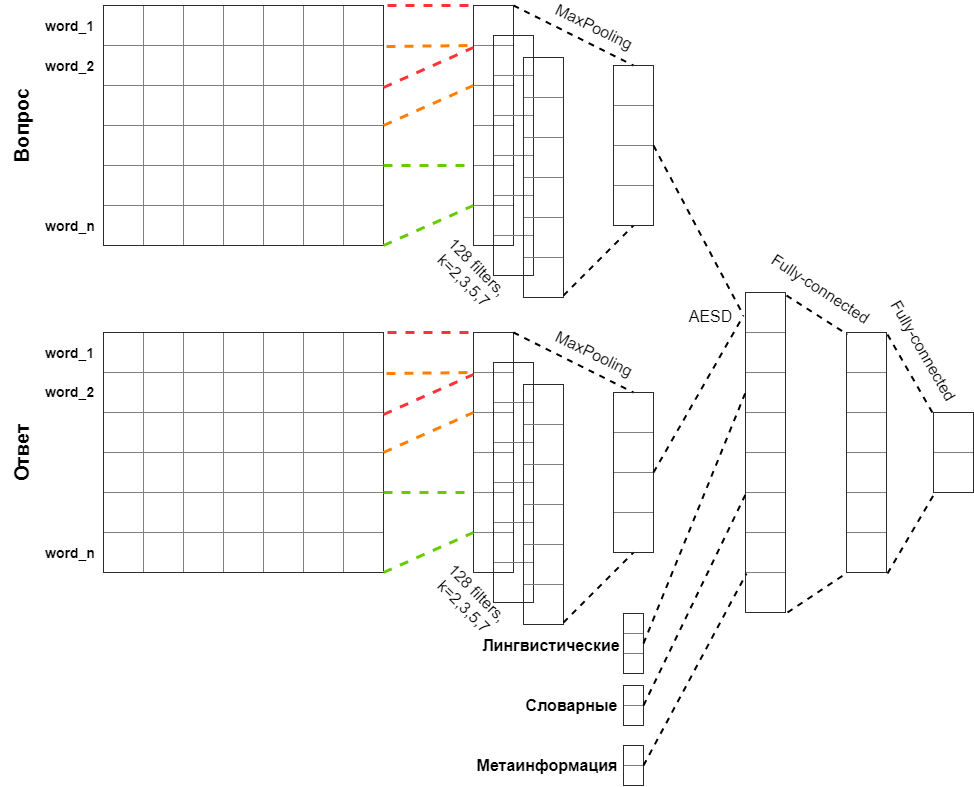
\includegraphics[width=0.9\linewidth]{images/my_cnn.png}
   		\captionof{figure}{Архитектура, основанная на сверточных слоях}
		\label{fig:my_cnn}
   	\end{figure}


	\subsubsection{Рекуррентная нейронная сеть}

	На рисунке \ref{fig:my_rnn} указана архитектура, основанная на рекуррентной сети.
	В качестве оптимальных параметров были использованы двунаправленная рекуррентная сеть с выходной размерностью, равной $128$, размер скрытого слоя равен $256$, 
	а коэффициент Dropout равен $0.5$.

   	\vskip 1em
    \begin{figure}[!ht]
   	    \centering
		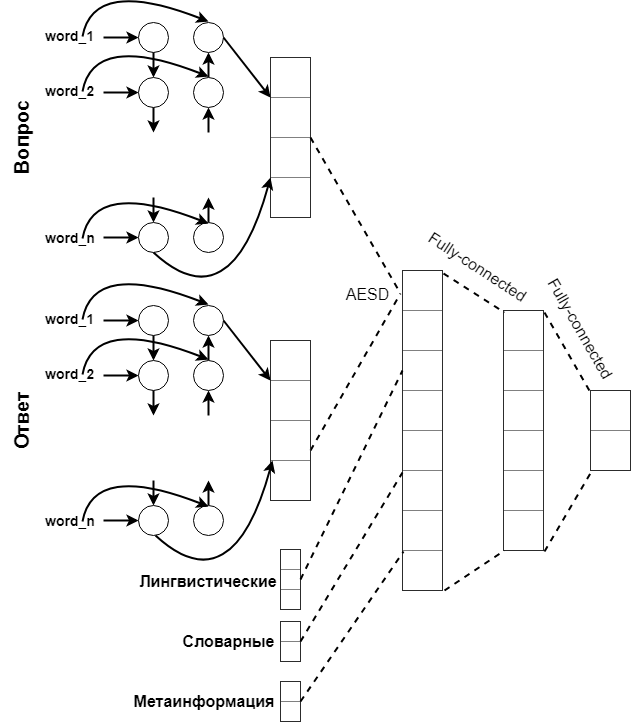
\includegraphics[width=0.9\linewidth]{images/my_rnn.png}
   		\captionof{figure}{Архитектура, основанная на рекуррентных слоях}
		\label{fig:my_rnn}
   	\end{figure}

   	Стоит отметить, что эта модель требует в разы больше времени на обучение, что объясняется наличием двунаправленного рекуррентного слоя.
	
	\subsubsection{Детали реализации}

 	Все вышеобозначенные модели и их модификации были реализованы с помощью фреймворка Keras \cite{online:keras}.

 	Для обучения и работы с моделями Word2Vec и Fasttext использовался фреймворк Gensim \cite{online:gensim}.

 	Для предобработки текста использовалась библиотека NLTK \cite{online:nltk}, 
 	а для извлечения различных лингвистических признаков была использована модификация библиотеки textstat \cite{online:textstat}.

 	\subsubsection{Репозиторий}

 	Исходный код доступен по ссылке \cite{online:repository}.

\end{document}

                                                                                                               